\documentclass[tikz,border=5pt]{standalone}
\usepackage{amsmath}
\usetikzlibrary{arrows.meta,calc}
\definecolor{ink}{HTML}{234675}
\definecolor{bluefill}{HTML}{DFEFFE}
\definecolor{greenfill}{HTML}{DEF6D6}
\definecolor{pinkfill}{HTML}{FCCCDA}
\begin{document}
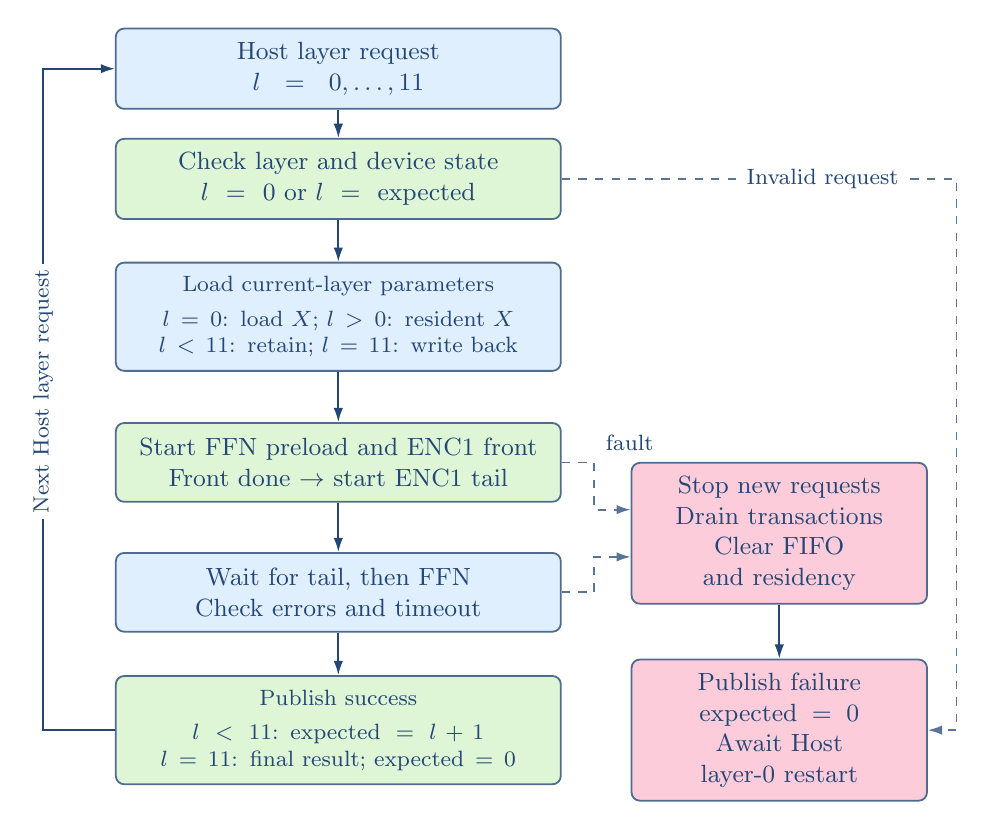
\begin{tikzpicture}[font=\small,text=ink,
 flowbox/.style={draw=ink!80,line width=.65pt,rounded corners=3pt,align=center,inner sep=5pt,text width=53mm,minimum height=10mm},
 arr/.style={-{Latex[length=1.8mm,width=1.2mm]},draw=ink,line width=.65pt},
 fault/.style={arr,draw=ink!75,dashed},
 tag/.style={font=\footnotesize,fill=white,inner sep=2pt}]
\node[flowbox,fill=bluefill] (request) at (0,0) {Host layer request\\$l=0,\ldots,11$};
\node[flowbox,fill=greenfill] (check) at (0,-1.4) {Check layer and device state\\$l=0$ or $l=\mathrm{expected}$};
\node[flowbox,fill=bluefill,font=\footnotesize] (config) at (0,-3.15) {Load current-layer parameters\\[3pt]
$l=0$: load $X$; $l>0$: resident $X$\\
$l<11$: retain; $l=11$: write back};
\node[flowbox,fill=greenfill] (execute) at (0,-5) {Start FFN preload and ENC1 front\\Front done $\rightarrow$ start ENC1 tail};
\node[flowbox,fill=bluefill] (wait) at (0,-6.65) {Wait for tail, then FFN\\Check errors and timeout};
\node[flowbox,fill=greenfill,font=\footnotesize] (success) at (0,-8.4) {Publish success\\[3pt]
$l<11$: $\mathrm{expected}=l+1$\\
$l=11$: final result; $\mathrm{expected}=0$};
\foreach \a/\b in {request/check,check/config,config/execute,execute/wait,wait/success}{\draw[arr] (\a.south)--(\b.north);}
\node[flowbox,fill=pinkfill,text width=34mm] (drain) at (5.6,-5.9) {Stop new requests\\Drain transactions\\Clear FIFO and residency};
\node[flowbox,fill=pinkfill,text width=34mm] (fail) at (5.6,-8.4) {Publish failure\\$\mathrm{expected}=0$\\Await Host layer-0 restart};
\draw[fault] (check.east)--(7.85,-1.4)--(7.85,-8.4)--(fail.east);
\node[tag,align=center] at (6.15,-1.4) {Invalid request};
\draw[fault] (execute.east)--(3.25,-5) |- ($(drain.west)+(0,.3)$);
\node[tag] at (3.7,-4.75) {fault};
\draw[fault] (wait.east)--(3.25,-6.65) |- ($(drain.west)+(0,-.3)$);
\draw[arr] (drain.south)--(fail.north);
\draw[arr] (success.west)--(-3.75,-8.4)--(-3.75,0)--(request.west);
\node[tag,rotate=90] at (-3.75,-4.1) {Next Host layer request};
\end{tikzpicture}
\end{document}

